\documentclass[11pt]{article}

\usepackage[margin=1in]{geometry}
\usepackage{amsmath,amssymb,booktabs,longtable,array}
\usepackage{enumitem}
\usepackage{float}
\usepackage[hidelinks]{hyperref}
\usepackage{listings}
\usepackage{microtype}
\usepackage{siunitx}
\usepackage{xcolor}
\usepackage{tikz}
\usetikzlibrary{arrows.meta,calc,fit,positioning,shapes.geometric}

\newcommand{\R}{\mathbb{R}}
\newcommand{\norm}[1]{\left\lVert #1\right\rVert_2}
\newcommand{\abs}[1]{\left\lvert #1\right\rvert}
\newcommand{\code}[1]{\texttt{#1}}
\newcommand{\measured}{\textsc{measured}}
\newcommand{\derived}{\textsc{derived}}
\newcommand{\planned}{\textsc{planned}}
\newcommand{\failed}{\textsc{failed}}
\newcolumntype{L}[1]{>{\raggedright\arraybackslash}p{#1}}
\newcolumntype{C}[1]{>{\centering\arraybackslash}p{#1}}
\DeclareSIUnit\barunit{bar}

\definecolor{trainingblue}{RGB}{38,92,140}
\definecolor{archivegold}{RGB}{183,126,20}
\definecolor{exactred}{RGB}{151,45,45}
\definecolor{acceptgreen}{RGB}{43,122,70}
\definecolor{lightgray}{RGB}{245,245,245}

\lstdefinestyle{reportlisting}{
  basicstyle=\ttfamily\small,
  columns=fullflexible,
  frame=single,
  framerule=0.3pt,
  breaklines=true,
  keepspaces=true,
  showstringspaces=false,
  xleftmargin=1em,
  xrightmargin=1em
}
\lstset{style=reportlisting}

\title{Offline Neural Surrogates for Thermochimica in MOOSE:\\
Mathematical Formulation, Safeguarded Deployment, and Prototype Evaluation}
\author{MOOSE Chemical Reactions Module}
\date{Technical report, 29 July 2026}

\begin{document}
\maketitle

\begin{abstract}
Thermochimica computes multiphase thermodynamic equilibrium through constrained Gibbs-energy
minimization.  Repeating that nonlinear calculation at every mesh entity can dominate a
MOOSE-based simulation.  This report presents a complementary acceleration path in which exact
Thermochimica states are generated offline, a deterministic multi-output neural network is trained
in PyTorch, and the resulting CPU TorchScript archive is evaluated in batches by isolated
Thermochimica worker processes.  The deployed map uses logarithmic temperature and pressure,
normalized elemental composition, embedded input and output standardization, and explicit
rescaling of extensive outputs.

The neural result is never treated as globally valid.  Archive schema version 2 binds the model
to the thermodynamic identity and adds phase-presence logits, calibrated per-assemblage
distance-to-training-support gates, inverse-transformed nonnegative outputs, and coupled
phase/element-fraction invariants.  Low-confidence or contradictory phase labels, unsupported
assemblages, nonfinite values, invariant violations, and audit-selected rows are evaluated
exactly.  Every audited row publishes the exact Thermochimica value, and the first failed audit
disables neural inference in that worker.

This revision changes the scientific qualification target.  The original smooth gas-bearing
trajectory is retained only as a \emph{legacy performance microbenchmark}; it is not headline
evidence for general fluoride chemistry.  \measured{} preliminary evidence includes a
\(24\times24\) exact Fe--Cr phase-map scan and an unrestricted eight-state
F--Li--U--Th--Ni--Nd--Ce--La--Cs--I discovery smoke test using
\code{MSDTC\_41\_fluorides.dat}.  Seven of those eight fluoride states contained MSFL plus a
non-gas condensed phase, and the discovered union included solid LiF, \code{Ni\_fcc(s)}, and
\code{U\_S1(s)} as well as MSFL and ideal gas.  The production-size phase maps, element-count
curves, trained NS replay archive, and acceptance timings remain \planned{} until the corresponding
held-out and repeated runs finish.  No preliminary number is promoted to a fluoride-wide
acceleration claim.
\end{abstract}

\tableofcontents

\section{Executive assessment}

The prototype establishes the complete offline-to-runtime path needed to use a PyTorch model as a
Thermochimica accelerator in MOOSE.  Its principal strengths are:
\begin{itemize}[leftmargin=*]
  \item exact Thermochimica remains the authority for data generation, runtime fallback, and
  periodic auditing;
  \item the archive is self-contained and is rejected when its thermodynamic identity or ordered
  input/output contract differs from the MOOSE configuration;
  \item one batched CPU forward call serves all eligible rows in a worker request;
  \item extensive and intensive outputs retain their distinct scaling laws;
  \item per-assemblage training-support, calibrated phase-confidence, physical output invariants,
  and finite-value checks are enforced before publication;
  \item an audit failure disables the model locally rather than allowing repeated unverified
  predictions; and
  \item exact, local inverse-distance, and KKT-linear modes remain available and do not require
  libtorch.
\end{itemize}

The earlier timing evidence remains useful for implementation performance, but its scientific
scope is narrow: the Fe--Cr archive covered one BCC region and the fluoride archive followed one
smooth MSFL/gas trajectory.  The revised campaign instead requires separate evidence for
single-phase interiors, multiphase interiors, and transition buffers, with transition ambiguity
treated as an intended exact fallback.

The current evidence status is explicit:
\begin{enumerate}[leftmargin=*]
  \item \measured: schema-2 unit tests, a libtorch MOOSE load/inference smoke test, a
  \(24\times24\) exact Fe--Cr scan, Li--F table replay, and the unrestricted ten-element
  fluoride discovery smoke test;
  \item \derived: the active fluoride output union and replay specification are generated from
  exact discovery values above \(10^{-10}\) per unit-total composition;
  \item \planned: the full \(64\times64/63\times63\) Fe--Cr grids, 9/13/17-element SLURM
  campaign, production \(48\times96\) NS fields, repeated timing, and confidence intervals;
  \item \failed: no acceptance criterion is marked failed merely because its run is unfinished;
  an actual tolerance, unseen-phase, or speed gate failure will remain in the final table; and
  \item TorchScript remains a version-coupled prototype deployment mechanism; a future PT2 loader
  must preserve the same archive-level thermodynamic contract.
\end{enumerate}

The defensible conclusion is therefore narrower than the original report: the phase-aware runtime
and qualification machinery are implemented, while general multiphase fluoride acceleration and
the NS speed target are not yet qualified.

\section{Problem statement and scope}

\subsection{Thermodynamic equilibrium map}

Let \(T>0\) and \(P>0\) denote temperature and pressure.  Let
\(\boldsymbol{a}=(a_1,\ldots,a_E)^T\in\R_{\geq0}^{E}\) contain the supplied elemental amounts.
Abstractly, Thermochimica computes
\begin{equation}
  \boldsymbol{n}^{\star}(T,P,\boldsymbol{a})
  \in \underset{\boldsymbol{n}\geq0}{\operatorname{argmin}}\;
  G(T,P,\boldsymbol{n})
  \quad\text{subject to}\quad
  \mathbf{A}\boldsymbol{n}=\boldsymbol{a},
  \label{eq:gem}
\end{equation}
where \(\boldsymbol{n}\) denotes phase and species amounts and \(\mathbf{A}\) is the elemental
incidence matrix.  A configured MOOSE object extracts an ordered vector
\begin{equation}
  \boldsymbol{y}
  =\mathcal{F}(T,P,\boldsymbol{a})
  =\left(y_1,\ldots,y_m\right)^T\in\R^m.
  \label{eq:exact-map}
\end{equation}
The entries can include system Gibbs energy, phase amounts, phase fractions, elemental potentials,
species chemical potentials, vapor pressures, constituent fractions, and other supported
Thermochimica outputs.

The equilibrium map is generally piecewise smooth.  Within a fixed active phase and constituent
set, a low-dimensional path can be smooth enough for accurate regression.  At a phase boundary,
the active constraints in Equation~\eqref{eq:gem} change; derivatives can be discontinuous and a
phase amount can become identically zero.  An offline surrogate must therefore be associated with
a declared training domain and guarded by exact fallback.

\subsection{Surrogate objective}

The deployed network approximates the requested output map,
\begin{equation}
  \widehat{\mathcal{F}}_{\boldsymbol{\theta}}:
  \mathcal{D}_{\mathrm{train}}\subset\R^{E+2}\longrightarrow\R^m,
  \qquad
  \widehat{\boldsymbol{y}}
  =\widehat{\mathcal{F}}_{\boldsymbol{\theta}}(T,P,\boldsymbol{a}),
  \label{eq:surrogate-map}
\end{equation}
where \(\boldsymbol{\theta}\) is fixed at runtime.  The optimization objective is not only small
regression error.  For a simulation with \(N\) thermochemical states, it is to reduce the number
of exact solves,
\begin{equation}
  N_{\mathrm{GEM,neural}}
  =N_{\mathrm{seed}}+N_{\mathrm{audit}}+N_{\mathrm{fallback}},
  \label{eq:exact-count}
\end{equation}
while retaining exact results on every safeguard path.

This prototype does not perform online retraining, uncertainty quantification, GPU inference,
global phase-diagram learning, or automatic sampling.  It also does not change
Equation~\eqref{eq:gem}; exact mode remains the reference calculation.

\section{End-to-end architecture}

Figure~\ref{fig:pipeline} separates offline training from online simulation.  The same output
descriptor ordering is carried through exact CSV generation, the JSON training specification,
archive metadata, the network output tensor, and the MOOSE result buffer.

\begin{figure}[p]
  \centering
  \resizebox{\textwidth}{!}{%
  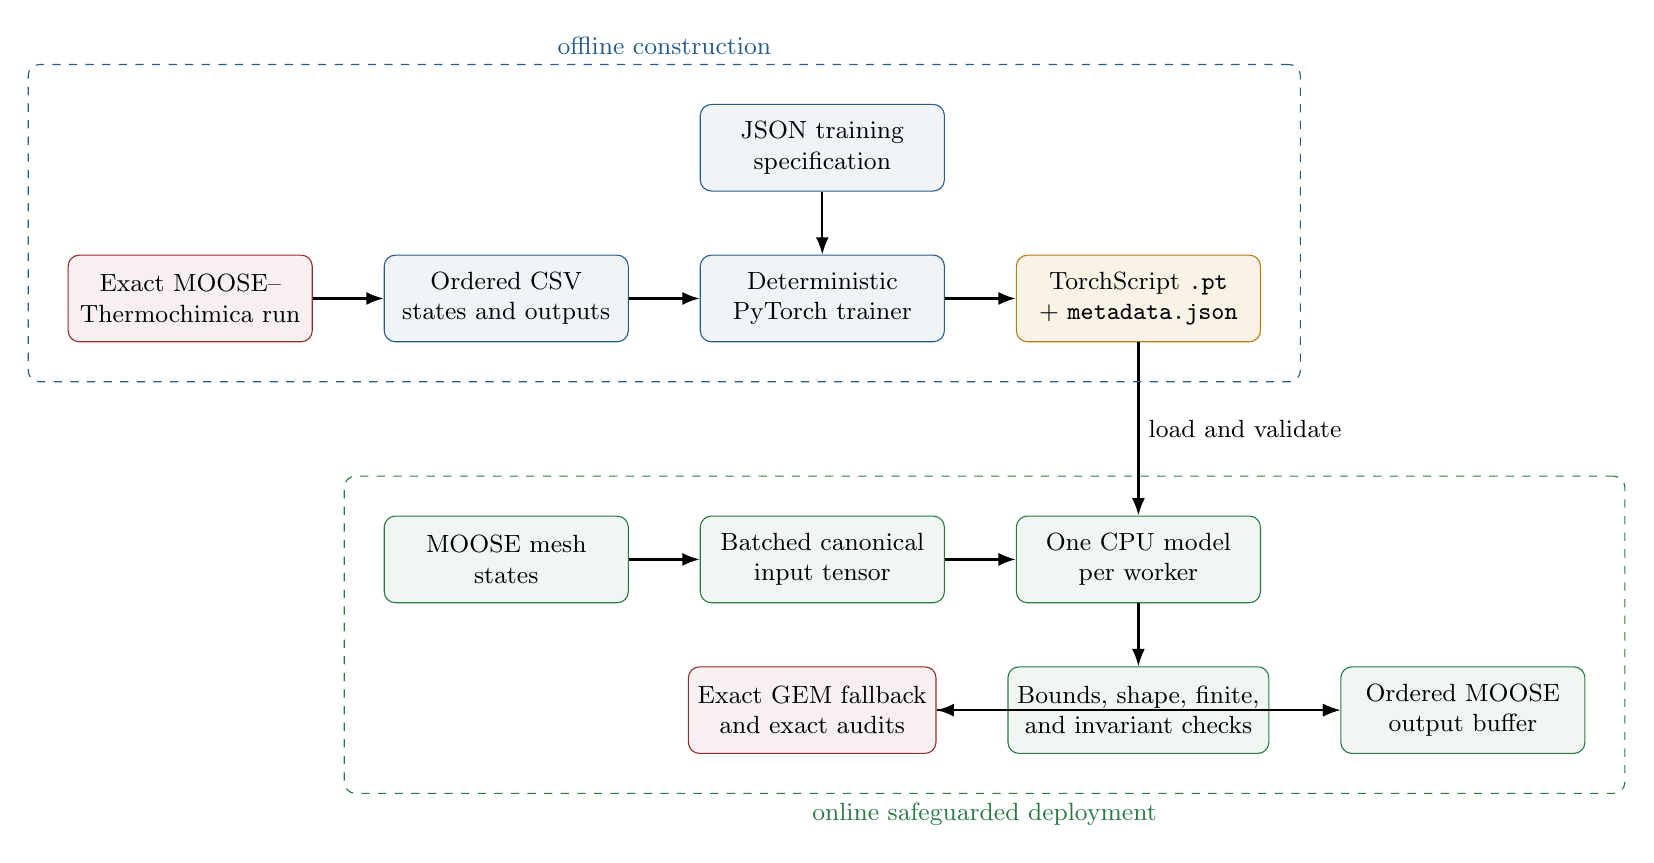
\begin{tikzpicture}[
    font=\small,
    node distance=8mm and 9mm,
    box/.style={draw, rounded corners, align=center, minimum height=11mm, minimum width=31mm},
    offline/.style={box, draw=trainingblue, fill=trainingblue!7},
    archive/.style={box, draw=archivegold, fill=archivegold!10},
    online/.style={box, draw=acceptgreen, fill=acceptgreen!7},
    exact/.style={box, draw=exactred, fill=exactred!7},
    arrow/.style={-{Latex[length=2.2mm]}, thick}
  ]
    \node[exact] (gem) {Exact MOOSE--\\Thermochimica run};
    \node[offline, right=of gem] (csv) {Ordered CSV\\states and outputs};
    \node[offline, right=of csv] (trainer) {Deterministic\\PyTorch trainer};
    \node[offline, above=of trainer] (spec) {JSON training\\specification};
    \node[archive, right=of trainer] (pt) {TorchScript \code{.pt}\\+\ \code{metadata.json}};

    \node[online, below=22mm of pt] (load) {One CPU model\\per worker};
    \node[online, left=of load] (batch) {Batched canonical\\input tensor};
    \node[online, left=of batch] (moose) {MOOSE mesh\\states};
    \node[online, below=of load] (guards) {Bounds, shape, finite,\\and invariant checks};
    \node[exact, left=of guards] (fallback) {Exact GEM fallback\\and exact audits};
    \node[online, right=of guards] (publish) {Ordered MOOSE\\output buffer};

    \draw[arrow] (gem) -- (csv);
    \draw[arrow] (csv) -- (trainer);
    \draw[arrow] (spec) -- (trainer);
    \draw[arrow] (trainer) -- (pt);
    \draw[arrow] (pt) -- node[right]{load and validate} (load);
    \draw[arrow] (moose) -- (batch);
    \draw[arrow] (batch) -- (load);
    \draw[arrow] (load) -- (guards);
    \draw[arrow] (guards) -- (publish);
    \draw[arrow] (guards) -- (fallback);
    \draw[arrow] (fallback) -- (publish);

    \node[draw=trainingblue, dashed, rounded corners,
          fit=(gem)(csv)(trainer)(spec)(pt), inner sep=5mm,
          label={[trainingblue]above:offline construction}] {};
    \node[draw=acceptgreen, dashed, rounded corners,
          fit=(moose)(batch)(load)(guards)(fallback)(publish), inner sep=5mm,
          label={[acceptgreen]below:online safeguarded deployment}] {};
  \end{tikzpicture}
  }
  \caption{Offline training and online MOOSE deployment.  The archive is the only artifact that
  crosses the two stages.}
  \label{fig:pipeline}
\end{figure}

\subsection{Offline construction}

An exact MOOSE input generates a CSV containing the raw temperature, pressure, elemental
compositions, and requested outputs.  A compact JSON file supplies the column interpretation,
database path, units, ordered elements, phase selection, ordered output descriptors, semantic
flags, training controls, and validation tolerances.  The trainer then:
\begin{enumerate}[leftmargin=*]
  \item converts raw states to the canonical representation;
  \item normalizes extensive responses to unit total composition;
  \item makes a seeded train/validation split;
  \item computes standardization statistics from training rows only;
  \item optimizes a fixed fully connected network;
  \item restores the best validation-loss state; and
  \item traces and saves the model together with archive metadata and a human-readable validation
  report.
\end{enumerate}

\subsection{Online execution}

Thermochimica uses stateful Fortran modules and is not reentrant.  The existing MOOSE executor
therefore forks isolated workers and transfers batched input and output arrays through shared
memory.  Each worker loads one CPU model, fixes PyTorch intra-operation threads to one, and makes
one forward call for all eligible rows in a received batch.  Model state and audit state are
worker-local; no neural-model lock is required.

This design gives two levels of parallelism: MOOSE distributes states among workers, while each
worker applies dense matrix operations over a batch.  It avoids oversubscription by not allowing
each worker's PyTorch runtime to create another thread team.

\section{Canonical thermodynamic representation}

\subsection{Inputs}

The total supplied composition is
\begin{equation}
  A=\sum_{i=1}^{E}a_i.
  \label{eq:total}
\end{equation}
For finite \(a_i\geq0\), \(A>0\), \(T_K>0\), and \(P_{\mathrm{bar}}>0\), the canonical input is
\begin{equation}
  \boldsymbol{z}
  =
  \left[
    \log\left(\frac{T_K}{T_{\mathrm{ref}}}\right),
    \log\left(\frac{P_{\mathrm{bar}}}{P_{\mathrm{ref}}}\right),
    x_1,\ldots,x_E
  \right]^T,
  \quad
  x_i=\frac{a_i}{A},
  \quad
  T_{\mathrm{ref}}=\SI{298.15}{\kelvin},
  \quad
  P_{\mathrm{ref}}=\SI{1}{\barunit}.
  \label{eq:canonical-input}
\end{equation}
Thus \(d=E+2\).  The logarithms make multiplicative temperature and pressure changes additive and
prevent a large dimensional scale difference from being carried directly into the network.
Composition magnitude is separated from composition ratios.

The present representation retains all \(E\) fractions even though
\(\sum_i x_i=1\).  It is easy to audit against the configured element ordering but contains one
redundant coordinate.  A future high-dimensional model could use \(E-1\) independent simplex
coordinates or a log-ratio representation, provided the archive schema records that change.

\subsection{Extensive output normalization}

Each output descriptor carries an extensivity flag \(e_j\in\{0,1\}\).  The target stored for
training is
\begin{equation}
  \bar y_j=\frac{y_j}{A^{e_j}}.
  \label{eq:extensive-normalization}
\end{equation}
At runtime, the physical prediction is reconstructed as
\begin{equation}
  \widehat y_j=A^{e_j}\widehat{\bar y}_j.
  \label{eq:extensive-rescaling}
\end{equation}
For an amount-based input, this encodes the degree-one homogeneity expected of total phase amounts
and total Gibbs energy:
\begin{equation}
  y_j(T,P,\lambda\boldsymbol{a})=\lambda y_j(T,P,\boldsymbol{a}),
  \qquad e_j=1,\quad\lambda>0.
  \label{eq:homogeneity}
\end{equation}
Potentials and fractions have \(e_j=0\) and are unchanged by a uniform composition scaling.  This
separation allows a network trained at unit total composition to serve other totals without
learning a trivial linear direction.

\section{Neural approximation and optimization}

\subsection{Embedded standardization}

Let the training subset have input mean \(\boldsymbol{\mu}_z\), componentwise input standard
deviation \(\boldsymbol{\sigma}_z\), normalized-output mean
\(\boldsymbol{\mu}_y\), and normalized-output standard deviation
\(\boldsymbol{\sigma}_y\).  Each scale is clamped below by \(10^{-12}\).  The model evaluates
\begin{align}
  \widetilde{\boldsymbol{z}}
    &=\left(\boldsymbol{z}-\boldsymbol{\mu}_z\right)
      \oslash\boldsymbol{\sigma}_z,
      \label{eq:input-standardization}\\
  \widehat{\bar{\boldsymbol{y}}}
    &=\boldsymbol{\mu}_y+
      \boldsymbol{\sigma}_y\odot
      f_{\boldsymbol{\theta}}(\widetilde{\boldsymbol{z}}),
      \label{eq:output-destandardization}
\end{align}
where \(\odot\) and \(\oslash\) are componentwise multiplication and division.  All four vectors
are registered as model buffers.  Consequently, the archive accepts physical canonical inputs
and returns physical normalized outputs; C++ does not reproduce Python preprocessing constants.

\subsection{Network architecture}

The regression network is
\begin{equation}
  d
  \xrightarrow{\mathrm{affine}}\!128
  \xrightarrow{\mathrm{SiLU}}\!128
  \xrightarrow{\mathrm{SiLU}}\!64
  \xrightarrow{\mathrm{SiLU}}\!m,
  \label{eq:architecture}
\end{equation}
with
\begin{equation}
  \operatorname{SiLU}(q)=q\,\operatorname{sigmoid}(q)
  =\frac{q}{1+\exp(-q)}.
  \label{eq:silu}
\end{equation}
For hidden layer \(\ell\),
\begin{equation}
  \boldsymbol{h}^{(\ell)}
  =\operatorname{SiLU}\left(
    \mathbf{W}^{(\ell)}\boldsymbol{h}^{(\ell-1)}
    +\boldsymbol{b}^{(\ell)}
  \right),
  \qquad
  \boldsymbol{h}^{(0)}=\widetilde{\boldsymbol{z}},
  \label{eq:hidden}
\end{equation}
and the last layer is affine.  Figure~\ref{fig:network} shows that standardization and
destandardization belong to the exported module rather than the MOOSE caller.

\begin{figure}[htbp]
  \centering
  \resizebox{0.98\textwidth}{!}{%
  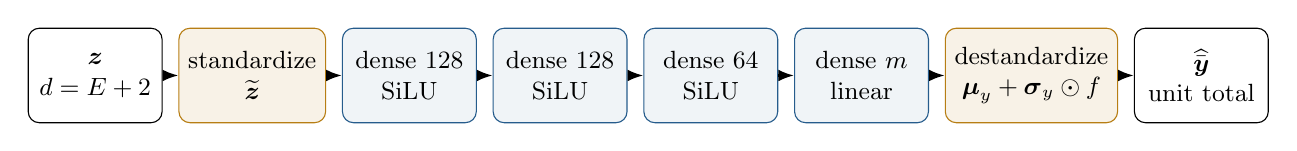
\begin{tikzpicture}[
    font=\small,
    node distance=2mm,
    layer/.style={draw, rounded corners, align=center, minimum height=12mm, minimum width=17mm},
    transform/.style={layer, fill=archivegold!10, draw=archivegold},
    dense/.style={layer, fill=trainingblue!7, draw=trainingblue},
    arrow/.style={-{Latex[length=2mm]}, thick}
  ]
    \node[layer] (input) {\(\boldsymbol{z}\)\\\(d=E+2\)};
    \node[transform, right=of input] (std) {standardize\\\(\widetilde{\boldsymbol{z}}\)};
    \node[dense, right=of std] (h1) {dense 128\\SiLU};
    \node[dense, right=of h1] (h2) {dense 128\\SiLU};
    \node[dense, right=of h2] (h3) {dense 64\\SiLU};
    \node[dense, right=of h3] (out) {dense \(m\)\\linear};
    \node[transform, right=of out] (destd) {destandardize\\\(\boldsymbol{\mu}_y+
      \boldsymbol{\sigma}_y\odot f\)};
    \node[layer, right=of destd] (result) {\(\widehat{\bar{\boldsymbol{y}}}\)\\unit total};

    \draw[arrow] (input) -- (std);
    \draw[arrow] (std) -- (h1);
    \draw[arrow] (h1) -- (h2);
    \draw[arrow] (h2) -- (h3);
    \draw[arrow] (h3) -- (out);
    \draw[arrow] (out) -- (destd);
    \draw[arrow] (destd) -- (result);
  \end{tikzpicture}
  }
  \caption{Exported multi-output network.  Runtime extensive rescaling from
  Equation~\eqref{eq:extensive-rescaling} follows the final node.}
  \label{fig:network}
\end{figure}

The number of trainable scalar parameters is
\begin{equation}
  N_{\theta}
  =(128d+128)+(128^2+128)+(64\cdot128+64)+(64m+m).
  \label{eq:parameter-count}
\end{equation}
This is 25,928 parameters for Fe--Cr (\(d=4,m=8\)) and 26,182 parameters for the fluoride case
(\(d=7,m=6\)).  The network is therefore small relative to typical deep-learning models; its
runtime value comes primarily from batched dense arithmetic and avoidance of nonlinear GEM.

\subsection{Training objective and deterministic split}

Given \(N\) exact rows, a NumPy random generator with the configured seed produces one permutation.
For validation fraction \(q\), the first
\begin{equation}
  N_v=\max\left(1,\operatorname{round}(qN)\right)
  \label{eq:validation-size}
\end{equation}
rows form the validation set and the remaining rows form the training set.  PyTorch is seeded with
the same integer before model construction.

The full training subset is used in each optimizer step.  With normalized targets
\(\bar{\boldsymbol{y}}_r\), the loss is
\begin{equation}
  \mathcal{L}_{\mathrm{train}}(\boldsymbol{\theta})
  =
  \frac{1}{N_t m}
  \sum_{r\in\mathcal{T}}
  \norm{
    \left(
      \widehat{\bar{\boldsymbol{y}}}_r-\boldsymbol{\mu}_y
    \right)\oslash\boldsymbol{\sigma}_y
    -
    \left(
      \bar{\boldsymbol{y}}_r-\boldsymbol{\mu}_y
    \right)\oslash\boldsymbol{\sigma}_y
  }^2.
  \label{eq:loss}
\end{equation}
Standardizing the response prevents a large-magnitude Gibbs energy or potential from dominating a
small phase fraction solely because of units.  Adam updates the weights.  A plateau scheduler
halves the learning rate, down to \(10^{-6}\), and early stopping restores the state with minimum
validation loss.  Improvement must exceed \(10^{-10}\) to reset patience.

\subsection{Reported validation errors}

For output \(j\) and validation row \(r\), define
\begin{align}
  \Delta_{rj}
    &=\abs{\widehat y_{rj}-y_{rj}},
    \label{eq:absolute-error}\\
  \rho_{rj}
    &=\frac{\Delta_{rj}}
      {\max\left(\abs{\widehat y_{rj}},\abs{y_{rj}},u_{\min}\right)},
    \label{eq:relative-error}\\
  \mathrm{pass}_{rj}
    &\Longleftrightarrow
    \Delta_{rj}
    \leq\varepsilon_{a,j}
    +\varepsilon_{r,j}
      \max\left(\abs{\widehat y_{rj}},\abs{y_{rj}}\right),
    \label{eq:validation-test}
\end{align}
where \(u_{\min}\) is the smallest positive floating-point number used by the report calculation.
Equation~\eqref{eq:relative-error} is not informative when the reference is zero: a
\(10^{-15}\)-scale prediction can have relative error one.  Absolute tolerances are therefore
essential for absent phases and small species amounts.

\section{Safeguarded runtime algorithm}

\subsection{Archive initialization}

Worker initialization loads the module on the CPU in evaluation mode and extracts
\code{metadata.json} from the TorchScript extra-files area.  It rejects the archive unless all of
the following match the MOOSE configuration:
\begin{itemize}[leftmargin=*]
  \item schema version and archive type;
  \item ordered element names;
  \item temperature, pressure, and composition units;
  \item SHA-256 digest of the exact thermodynamic database bytes;
  \item phase-selection mode and ordered selected phases;
  \item number and order of outputs;
  \item output type and selectors such as phase, element, species, or constituent; and
  \item extensive, nonnegative, and fraction flags.
\end{itemize}
The canonical lower and upper bound vectors must both have width \(d\).  A mismatch is a parameter
error before equilibrium evaluation begins.

\subsection{Eligibility and inference}

The archive stores the coordinatewise box
\begin{equation}
  \mathcal{B}
  =\left\{
    \boldsymbol{z}\in\R^d:
    \boldsymbol{\ell}-\boldsymbol{\delta}
    \leq\boldsymbol{z}
    \leq\boldsymbol{u}+\boldsymbol{\delta}
  \right\},
  \label{eq:box}
\end{equation}
where \(\boldsymbol{\ell}\) and \(\boldsymbol{u}\) are training-data minima and maxima.  The
implementation uses
\begin{equation}
  \delta_k
  =10^{-6}\max\left(1,\abs{\ell_k},\abs{u_k}\right)
  \label{eq:bound-padding}
\end{equation}
to avoid rejecting a state due only to a float-conversion boundary.  Invalid canonical inputs and
rows outside \(\mathcal{B}\) bypass inference and run exact GEM.

All eligible inputs in a worker batch form a float32 tensor
\(\mathbf{Z}\in\R^{B_e\times d}\).  One model call gives
\begin{equation}
  \widehat{\mathbf{Y}}
  =\widehat{\mathcal{F}}_{\boldsymbol{\theta}}(\mathbf{Z})
  \in\R^{B_e\times m}.
  \label{eq:batch-forward}
\end{equation}
The tensor shape must match Equation~\eqref{eq:batch-forward}.  Each extensive column is rescaled
by its row total \(A_r\).

\subsection{Physical invariants}

For a configured nonnegative output,
\begin{equation}
  \widehat y_{rj}\geq0,
  \label{eq:nonnegative}
\end{equation}
and for a fraction,
\begin{equation}
  0\leq\widehat y_{rj}\leq1.
  \label{eq:fraction}
\end{equation}
Finite negative values in \([-10^{-10},0)\) are clamped to zero, and fraction values in
\((1,1+10^{-10}]\) are clamped to one.  Any larger violation or any nonfinite output rejects that
row.

For nonnegative outputs spanning many decades, training uses the declared invertible transform
\begin{equation}
  q_j(y)=\log\left(1+\frac{y}{s_j}\right),
  \qquad
  q_j^{-1}(v)=s_j\left(e^v-1\right),
  \label{eq:log1p-transform}
\end{equation}
where \(s_j>0\) is stored per output.  The inverse is embedded in the exported model, so the C++
runtime, invariants, audits, and published variables always operate on physical values.  Gibbs
energies and potentials retain the linear transform.

\subsection{Phase classification and per-assemblage support}

Let \(p_k(\boldsymbol{z})=\sigma(l_k/\tau)\) be the calibrated probability that phase \(k\) is
present, where \(l_k\) is a classifier logit and \(\tau>0\) is selected on the disjoint validation
file.  The predicted phase signature is
\begin{equation}
  \widehat{\boldsymbol{s}}(\boldsymbol{z})
  =\left(\mathbb{1}[p_1\geq\tfrac12],\ldots,
          \mathbb{1}[p_K\geq\tfrac12]\right).
  \label{eq:phase-signature}
\end{equation}
Every phase decision must satisfy
\begin{equation}
  \max(p_k,1-p_k)\geq c_{\min}=0.99,
  \label{eq:phase-confidence}
\end{equation}
and it must agree with the independently regressed phase amount relative to the configured
presence threshold.  Failure of either condition sends the row to exact GEM.

Coordinatewise bounds alone admit empty corners of a high-dimensional box.  Let
\(\widetilde{\boldsymbol{z}}\) be the network-standardized input and let
\(\mathcal{A}_{\boldsymbol{s}}\) contain standardized training anchors having signature
\(\boldsymbol{s}\).  Schema 2 exports one distance column per validation-calibrated assemblage:
\begin{equation}
  d_{\boldsymbol{s}}(\boldsymbol{z})
  =\min_{\boldsymbol{a}\in\mathcal{A}_{\boldsymbol{s}}}
    \norm{\widetilde{\boldsymbol{z}}-\boldsymbol{a}}.
  \label{eq:assemblage-distance}
\end{equation}
To bound archive size and the temporary
\(N_{\mathrm{batch}}\times N_{\mathrm{anchor}}\times d\) distance tensor, the implementation
retains at most 4096 anchors by default, stratified equally across calibration assemblages and
selected deterministically in training-table order.  The retained anchor count and the larger
number of represented training rows are both recorded.  Radius calibration uses the retained
set, so compression can only enlarge the measured validation distances and cannot silently use
the discarded points at deployment.
For validation distances \(D_{\boldsymbol{s}}\), the support radius is
\begin{equation}
  r_{\boldsymbol{s}}
  =\gamma\,Q_{0.99}(D_{\boldsymbol{s}}),\qquad \gamma=1.25,
  \label{eq:support-radius}
\end{equation}
subject to a small positive numerical floor.  A predicted signature absent from the calibrated
assemblage table, or a state with
\(d_{\widehat{\boldsymbol{s}}}>r_{\widehat{\boldsymbol{s}}}\), is rejected.  Thus a point can be
inside every marginal bound and still correctly fall back because it is far from training support.

\subsection{Coupled invariants}

Metadata defines complete groups of physical fraction outputs.  For a phase-fraction group
\(\mathcal{J}_{p}\) and each complete element-distribution group
\(\mathcal{J}_{e}\), acceptance requires
\begin{equation}
  \abs{\sum_{j\in\mathcal{J}_{p}}\widehat y_j-1}\leq10^{-3},
  \qquad
  \abs{\sum_{j\in\mathcal{J}_{e}}\widehat y_j-1}\leq10^{-3}.
  \label{eq:coupled-invariants}
\end{equation}
The runtime does not renormalize a failed prediction, because projection could hide a
thermodynamically inconsistent network result.  It executes exact Thermochimica instead.

\subsection{Exact seeding and audits}

When the exact warm-start strategy is \code{previous\_solve}, the first state received by a worker
is solved exactly.  This seeds Thermochimica's worker-local continuation branch before predictions
are introduced.

Let \(M\) be \code{surrogate\_audit\_interval}.  Every \(M\)th accepted prediction in a worker is
recomputed exactly.  Runtime auditing applies
\begin{equation}
  \abs{\widehat y_j-y_j^{\mathrm{exact}}}
  \leq
  \varepsilon_{a,j}
  +\varepsilon_r
   \max\left(\abs{\widehat y_j},\abs{y_j^{\mathrm{exact}}}\right),
  \label{eq:audit}
\end{equation}
where the MOOSE input's global \(\varepsilon_r\) and per-output \(\varepsilon_{a,j}\) are
authoritative.  The per-output tolerances stored in the training report are descriptive validation
criteria; they do not override the runtime input.

An audited row always publishes \(\boldsymbol{y}^{\mathrm{exact}}\), regardless of whether the
comparison passes.  On the first failure, the worker records the first failing output, prediction,
exact value, and tolerance, then disables neural inference for the rest of the run.  Other workers
continue under their own audit state.

\subsection{Control flow}

Figure~\ref{fig:runtime-flow} shows the per-batch decision structure.  Exact fallback is also used
if the forward call throws or returns an incorrectly shaped tensor.

\begin{figure}[p]
  \centering
  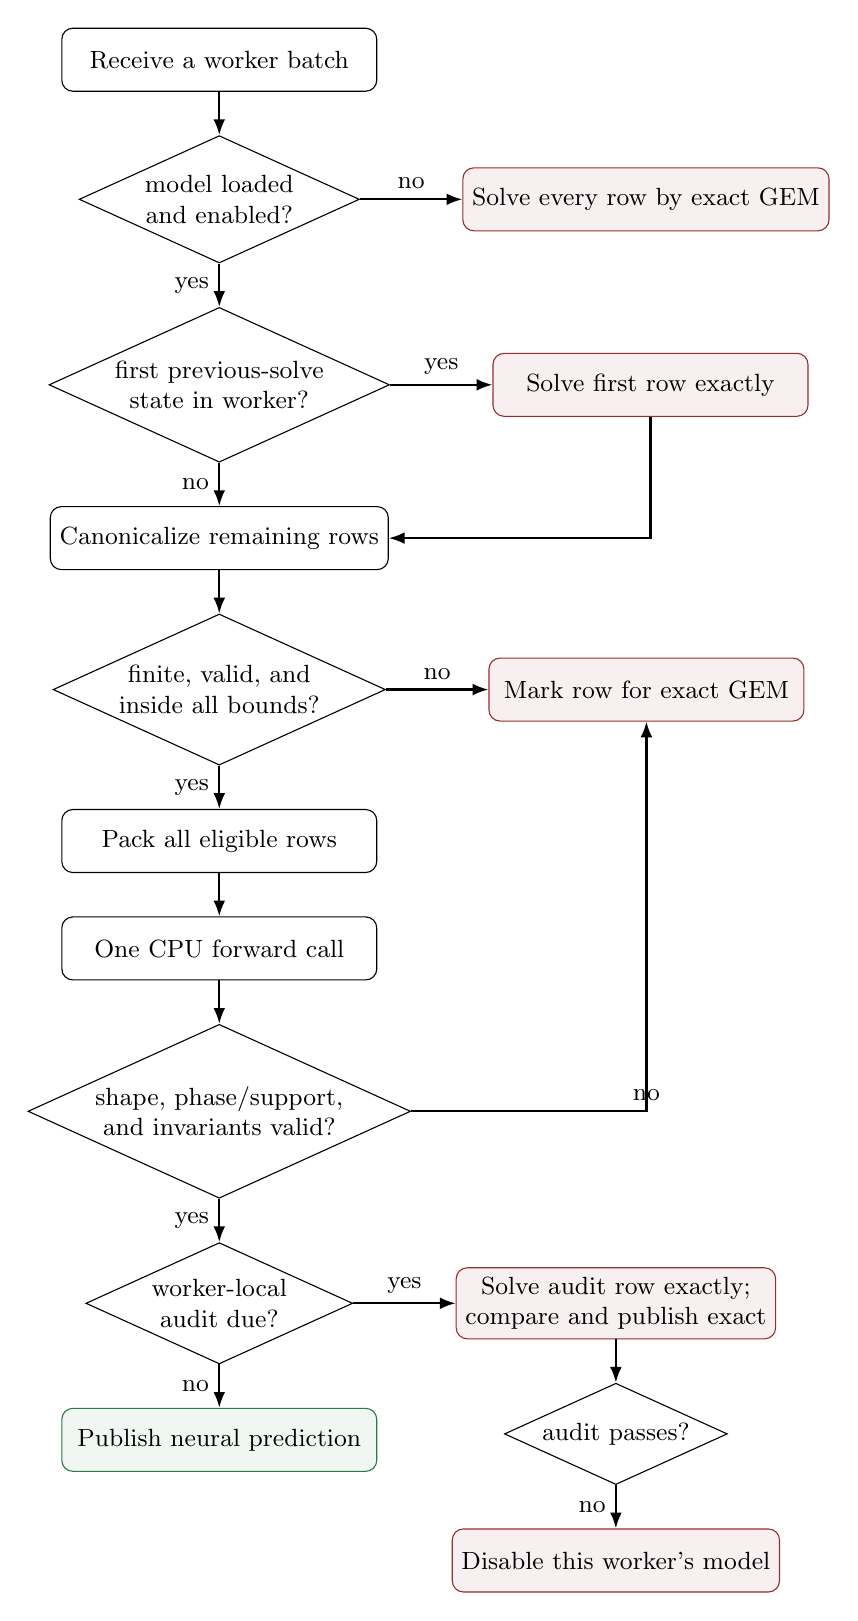
\begin{tikzpicture}[
    font=\small,
    node distance=5.5mm and 13mm,
    box/.style={draw, rounded corners, align=center, minimum width=40mm, minimum height=8mm},
    decision/.style={draw, diamond, aspect=2.2, align=center, inner sep=1.5pt},
    exact/.style={box, draw=exactred, fill=exactred!7},
    accepted/.style={box, draw=acceptgreen, fill=acceptgreen!7},
    arrow/.style={-{Latex[length=2mm]}, thick}
  ]
    \node[box] (receive) {Receive a worker batch};
    \node[decision, below=of receive] (enabled) {model loaded\\and enabled?};
    \node[exact, right=of enabled] (allgem) {Solve every row by exact GEM};
    \node[decision, below=of enabled] (seed) {first previous-solve\\state in worker?};
    \node[exact, right=of seed] (seedgem) {Solve first row exactly};
    \node[box, below=of seed] (canonical) {Canonicalize remaining rows};
    \node[decision, below=of canonical] (bounds) {finite, valid, and\\inside all bounds?};
    \node[exact, right=of bounds] (rowgem) {Mark row for exact GEM};
    \node[box, below=of bounds] (tensor) {Pack all eligible rows};
    \node[box, below=of tensor] (forward) {One CPU forward call};
    \node[decision, below=of forward] (valid) {shape, phase/support,\\and invariants valid?};
    \node[decision, below=of valid] (audit) {worker-local\\audit due?};
    \node[exact, right=of audit] (auditgem) {Solve audit row exactly;\\compare and publish exact};
    \node[accepted, below=of audit] (publish) {Publish neural prediction};
    \node[decision, below=of auditgem] (pass) {audit passes?};
    \node[exact, below=of pass] (disable) {Disable this worker's model};

    \draw[arrow] (receive) -- (enabled);
    \draw[arrow] (enabled) -- node[above]{no} (allgem);
    \draw[arrow] (enabled) -- node[left]{yes} (seed);
    \draw[arrow] (seed) -- node[above]{yes} (seedgem);
    \draw[arrow] (seed) -- node[left]{no} (canonical);
    \draw[arrow] (seedgem) |- (canonical);
    \draw[arrow] (canonical) -- (bounds);
    \draw[arrow] (bounds) -- node[above]{no} (rowgem);
    \draw[arrow] (bounds) -- node[left]{yes} (tensor);
    \draw[arrow] (tensor) -- (forward);
    \draw[arrow] (forward) -- (valid);
    \draw[arrow] (valid) -| node[above]{no} (rowgem);
    \draw[arrow] (valid) -- node[left]{yes} (audit);
    \draw[arrow] (audit) -- node[above]{yes} (auditgem);
    \draw[arrow] (audit) -- node[left]{no} (publish);
    \draw[arrow] (auditgem) -- (pass);
    \draw[arrow] (pass) -- node[left]{no} (disable);
  \end{tikzpicture}
  \caption{Safeguarded worker-batch evaluation.  Exact results fill every rejected, seed, and
  audit row.}
  \label{fig:runtime-flow}
\end{figure}

\subsection{Reference pseudocode}

Listing~\ref{lst:training} expresses the trainer at the level needed to reproduce its numerical
decisions.

\begin{lstlisting}[caption={Deterministic training and archive export.},label={lst:training}]
training = read_exact_moose_csv()
validation = read_disjoint_exact_validation_csv()
spec = read_json_specification()
z, total = canonicalize(T, P, ordered_element_columns)
y_bar = transform(normalize_extensive_outputs(y, total, output_flags))
phase_labels = presence_labels(y_bar, declared_phase_thresholds)
statistics = means_and_clamped_standard_deviations(training)
model = Standardize -> 128-SiLU -> 128-SiLU -> 64-SiLU
        -> regression + phase logits + per-assemblage support distances

repeat until epoch limit or early stopping:
    update model with Adam on standardized MSE + weighted phase BCE
    evaluate the same loss only on the explicit validation file
    update plateau scheduler
    retain best model and reset patience only on improvement > 1e-10

calibrate phase temperature and per-assemblage support radii on validation
metadata = ordered_contract + training_bounds + output transforms
           + phase/support gates + coupled invariants + validation metrics
trace_best_model_with_float32_example()
save_torchscript(model, extra_file={"metadata.json": metadata})
write_human_readable_validation_report()
\end{lstlisting}

Listing~\ref{lst:inference} emphasizes that batch inference is performed once, followed by
row-level acceptance.

\begin{lstlisting}[caption={Neural evaluation of one worker batch.},label={lst:inference}]
mark every row unresolved
if model is unavailable or disabled:
    solve every row exactly
    return

if previous_solve warm start has no worker history:
    solve first row exactly

for each remaining row:
    if canonical input is invalid or outside archive bounds:
        leave row unresolved
    else:
        append row to eligible tensor

prediction = one_forward_call(eligible_tensor)
require prediction shape == [eligible_rows, schema_declared_model_width]
for each predicted row:
    inverse-transform and rescale extensive regression outputs
    clamp only roundoff-sized invariant excursions
    classify phases and require confidence >= 0.99
    select matching assemblage support distance and radius
    if phase/regression labels disagree or support is absent:
        leave row unresolved
    else if any value is nonfinite or violates a scalar/coupled invariant:
        leave row unresolved
    else if audit is due:
        solve exactly, publish exact, compare all outputs
        disable this worker on any tolerance failure
    else:
        publish prediction

solve every unresolved row exactly
\end{lstlisting}

\section{Archive contract and deployment compatibility}

\subsection{Schema}

Table~\ref{tab:metadata} summarizes the compatible schema versions.  Metadata is embedded inside the
TorchScript ZIP container rather than stored as an adjacent file, so moving the archive does not
separate it from its contract.

\begin{longtable}{L{0.25\textwidth}L{0.27\textwidth}L{0.40\textwidth}}
  \caption{Embedded \code{metadata.json} fields.}
  \label{tab:metadata}\\
  \toprule
  Field & Purpose & Runtime treatment \\
  \midrule
  \endfirsthead
  \toprule
  Field & Purpose & Runtime treatment \\
  \midrule
  \endhead
  \code{schema\_version} &
  Selects the loader contract &
  Version 1 retains the original regression-only loader; version 2 enables the phase-aware
  layout. \\
  \code{archive\_type} &
  Distinguishes this artifact from an arbitrary TorchScript model &
  Must equal \code{thermochimica\_neural\_torchscript}. \\
  \code{database\_sha256} &
  Cryptographic identity of thermodynamic data &
  Must equal the digest computed from the configured file. \\
  \code{elements} &
  Ordered network composition columns &
  Must exactly equal configured names and order. \\
  input unit fields &
  Conversion interpretation for \(T,P,\boldsymbol{a}\) &
  Temperature, pressure, and composition units must match. \\
  \code{thermodynamic\_units} &
  J, J/mol, dimensionless fractions, configured pressure unit, and unit-total training basis &
  Records physical publication/audit semantics; configured input units remain the mismatch gate. \\
  \code{phase\_selection} &
  Included/excluded phase configuration &
  Mode and ordered phase list must match. \\
  \code{outputs} &
  Ordered semantic output descriptors and flags &
  Count, selectors, variable names, and semantic flags must match. \\
  \code{input\_lower\_bounds}, \code{input\_upper\_bounds} &
  Coordinatewise training envelope &
  Width must equal \(d\); every inferred row must lie inside. \\
  \code{model\_output\_layout} &
  Separates regression, phase-logit, and support-distance columns &
  Version-2 offsets/counts must be contiguous and match the model tensor width. \\
  \code{phase\_gate} &
  Presence outputs, thresholds, calibration temperature, and confidence &
  Each amount output and logit is validated before inference. \\
  \code{support.assemblages} &
  Signatures, distance columns, anchor counts, and calibrated radii &
  The classified row must match one entry and lie inside its radius. \\
  \code{invariant\_groups} &
  Complete phase and element-distribution fraction groups &
  Physical inverse-transformed sums must meet the declared target/tolerance. \\
  \code{torch\_version} &
  Export provenance &
  Recorded for diagnosis; compatibility is ultimately tested by load. \\
  \code{validation\_loss}, \code{validation\_metrics} &
  Training report &
  Informational at runtime; not an acceptance override. \\
  \bottomrule
\end{longtable}

\subsection{Public MOOSE interface}

The runtime selection is intentionally small:
\begin{lstlisting}[caption={MOOSE neural-surrogate selection.}]
[ChemicalComposition]
  [thermo]
    acceleration = adaptive
    surrogate_model = neural
    surrogate_archive = fe_cr.pt
    surrogate_relative_tolerance = 1e-3
    surrogate_absolute_tolerances = 'bcc_amount:1e-6'
    surrogate_audit_interval = 20
  []
[]
\end{lstlisting}

If \code{surrogate\_model=neural} is selected without an archive, input validation produces a
parameter error.  If MOOSE was built without libtorch, the same selection reports that the neural
surrogate requires libtorch support.  Neither condition changes exact or existing adaptive modes.

\subsection{TorchScript choice and future loader}

TorchScript is deprecated by PyTorch in favor of newer export and compilation paths.  It is used
for this prototype because MOOSE already has a tested C++ libtorch loader and TorchScript packages
the standardization buffers and metadata in one file.  The alternative AOTInductor C++ deployment
path creates a stronger coupling among compiler, PyTorch runtime, target platform, and generated
artifacts.  A future schema can select a different internal loader while retaining
\code{surrogate\_archive} as the MOOSE input parameter.  The archive type must remain explicit;
silently trying multiple loaders would weaken failure diagnosis.

\section{Implementation details}

\subsection{Repository components}

\begin{longtable}{L{0.36\textwidth}L{0.56\textwidth}}
  \caption{Principal implementation components.}
  \label{tab:components}\\
  \toprule
  Component & Responsibility \\
  \midrule
  \endfirsthead
  \toprule
  Component & Responsibility \\
  \midrule
  \endhead
  \code{ChemicalCompositionAction.C} &
  Adds the \code{neural} enum and archive parameter, preserves exact as the default, enforces
  libtorch capability, and transfers configuration. \\
  \code{ThermochimicaConfiguration.h} &
  Stores the neural model selection and archive path alongside ordered inputs, outputs,
  tolerances, units, and phase selection. \\
  \code{ThermochimicaData.C/.h} &
  Loads and validates one model per worker, builds batched tensors, applies bounds,
  per-assemblage support, phase gates, scalar/coupled invariants, schedules audits, executes exact
  fallback, disables failed workers, and reports telemetry. \\
  \code{train\_thermochimica\_nn.py} &
  Reads exact CSV and JSON, constructs canonical data, trains the fixed network, embeds metadata,
  exports TorchScript, and writes the validation report. \\
  \code{fe\_cr\_multiphase.i/.json} &
  Define the broad Fe--Cr phase map, BCC/FCC/HCP/liquid/sigma outputs, phase labels, transforms,
  and complete phase-fraction invariant. \\
  \code{element\_scaling.i/.json} &
  Hold the output vector fixed while the qualification driver changes nested element sets. \\
  \code{fluoride\_discovery.i} and \code{msfr\_compositions.csv} &
  Perform unrestricted ten-element discovery and preserve attributed early/depleted composition
  endpoints. \\
  \code{msfr\_ns\_precursor.i} and \code{msfr\_replay.i} &
  Generate a self-contained FV temperature/pressure field, then replay exact or neural
  thermochemistry with the discovery-active output union. \\
  \code{qualification.py} and \code{manifests/*.json} &
  Generate seeded Sobol states, run quick/full studies, train with explicit validation data,
  inspect active Exodus outputs, score the raw archive separately from guarded replay, reduce
  telemetry, repeat timings, and persist compact summaries. \\
  \code{plot\_qualification.py} &
  Generate exact Fe--Cr phase maps, element-scaling curves, MSFR field/error maps, and exact versus
  guarded-neural iodine inventory figures from an external result directory. \\
  \code{test\_trainer.py} and MOOSE test entries &
  Exercise export metadata plus capability-gated runtime behavior. \\
  \bottomrule
\end{longtable}

\subsection{Batch memory layout}

For a worker request of \(B\) rows, raw state arrays are already present in shared memory.  Eligible
rows are compacted into a contiguous float vector of length \(B_e d\), cloned into a Torch tensor,
and evaluated under inference mode.  Predictions are made contiguous on the CPU before indexed
access.  The additional transient storage is
\begin{equation}
  O(B_e d+B_e m)
  \label{eq:batch-memory}
\end{equation}
scalars, in addition to one copy of \(N_{\theta}\) model parameters per worker.

\subsection{Telemetry}

The existing performance report is extended with:
\begin{itemize}[leftmargin=*]
  \item \code{neural\_batches}: successful batched forward calls;
  \item \code{surrogate\_hits}: valid neural rows, including rows subsequently audited;
  \item \code{neural\_out\_of\_bounds}: valid canonical states outside the archive box;
  \item \code{neural\_support\_rejections}: in-box states outside calibrated assemblage support;
  \item \code{neural\_phase\_rejections}: low-confidence or regression-inconsistent phase labels;
  \item \code{invariant} and \code{error} rejections: bad values or inference-level failure;
  \item \code{audits} and \code{audit\_failures};
  \item \code{neural\_disabled\_workers};
  \item \code{neural\_inference\_time}; and
  \item exact solves, GEM iterations, worker solve time, packing time, and communication time.
\end{itemize}
Worker solve time and neural inference time are aggregated over workers.  They can exceed elapsed
wall time when several workers execute concurrently.  End-to-end wall time must therefore be
reported separately.

\subsection{Build and runtime coupling}

The prototype was compiled with MOOSE's libtorch option against PyTorch/libtorch 2.10 CPU
artifacts, matching the PyTorch 2.10 training environment.  This version matching is operationally
important: TorchScript provides serialization compatibility, but arbitrary mixtures of C++ and
Python distribution versions are not a supported deployment strategy.  The model is loaded once
per forked worker after process creation, avoiding unsafe reuse of a pre-fork runtime thread pool.

\section{Experimental methodology}

\subsection{Evidence classes}

\begin{longtable}{L{0.19\textwidth}L{0.31\textwidth}L{0.42\textwidth}}
  \caption{Evidence classes used in this report.}
  \label{tab:evidence}\\
  \toprule
  Class & Source & Permitted interpretation \\
  \midrule
  \endfirsthead
  \toprule
  Class & Source & Permitted interpretation \\
  \midrule
  \endhead
  Implementation fact &
  C++, Python, MOOSE input, and JSON at parent revision \code{6b1672b93b} plus the uncommitted
  neural-surrogate branch changes &
  Supports algorithm and control-flow statements; does not establish accuracy or speed. \\
  Trainer validation &
  Embedded archive report from an explicit disjoint exact CSV &
  Controls early stopping and calibration without spatially adjacent random-split leakage. \\
  Independent test &
  Exact CSV withheld from both optimization and calibration &
  Determines scientific acceptance; it is opened only by the benchmark driver after export. \\
  Runtime validation &
  Exact audits and exact-versus-neural state counters &
  Supports the observed guarded execution path and in-run error checks. \\
  Local timing &
  One development run per exact/neural configuration on macOS arm64 &
  Supports prototype order-of-magnitude comparisons only; no confidence interval or portable
  performance claim. \\
  \bottomrule
\end{longtable}

All numerical rows below are marked \measured\ when read from exact output, validation reports, or
MOOSE performance output.  Ratios marked \derived\ are arithmetic combinations of those measured
values.  Configured but unfinished values are \planned; failed gates are \failed{} and are not
silently removed.  No production HPC neural-surrogate campaign has been completed.

The driver performs two deliberately different comparisons.  First, it evaluates the exported
archive directly on the inaccessible test CSV before any MOOSE fallback can replace a bad
prediction.  These raw predictions determine scientific error and the smallest passing
element-scaling prefix.  Second, it replays the same states through MOOSE and reports published
outputs, gate-specific rejections, audits, exact solves, inference time, worker time, wall time,
and peak reported memory.  This prevents an all-fallback run from appearing to be an accurate
surrogate merely because its published values are exact.

\subsection{Multiphase, scaling, and NS campaign}

The Fe--Cr qualification domain is \(900\)--\(1800~\si{\kelvin}\), \(1~\si{\barunit}\), and
\(x_{\mathrm{Cr}}\in[0.02,0.98]\).  The quick grids are \(24\times24\) training,
\(12\times12\) disjoint validation, and \(23\times23\) staggered test; production uses
\(64\times64\), \(32\times32\), and \(63\times63\), respectively.  Validation calibrates early
stopping and support radii but is not reported as a test.  A case does not qualify as multiphase
unless exact results contain at least two assemblages and the production held-out set contains at
least 50 states with two phases above \(10^{-8}\) mole fraction.

The fluoride discovery samples five independent Sobol coordinates: \(T\), \(P\), depletion
interpolation, a fluorine factor in \([0.95,1.05]\), and a Ni factor in \([0.5,2]\).  It requests
\code{ALL} equilibrium phases and species from \code{MSDTC\_41\_fluorides.dat}; the active union is
selected at
\begin{equation}
  n_{\mathrm{active}}>\max(10^{-12}\ {\rm mol},10^{-10}n_{\mathrm{total}}).
\end{equation}
MSFL plus ideal gas alone is insufficient: at least one discovery state must contain MSFL and a
non-gas phase.  The element-scaling study separately uses nested 2/5/9/13/17-element sets,
independent composition coordinates, and a fixed output vector, so it measures computational
dimension rather than reactor realism.

Figure~\ref{fig:ns-workflow} shows the one-way-coupled NS methodology.  It is inspired by the VTB
MSFR thermochemistry workflow~\cite{vtbthermo} but is not a numerical reproduction: the present
precursor, database, mesh, and composition policy differ.  The attributed composition table sums
isotopes from the VTB depletion CSV.  Because its earliest row is at five days, the local
\code{fresh\_proxy} retains the ten element-wise isotope sums from that row; it is not labeled an
exact zero-burnup VTB fresh state.  The local 1~mol\% Ni corrosion inventory is likewise an explicit benchmark
assumption.

\begin{figure}[H]
  \centering
  \resizebox{\textwidth}{!}{%
  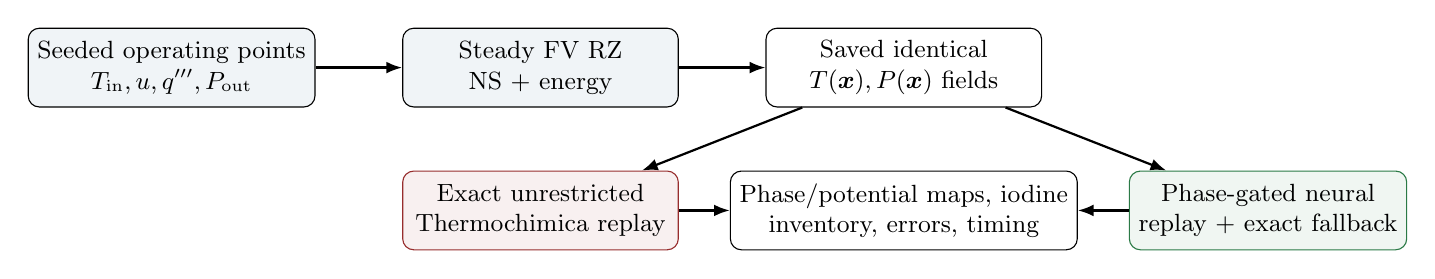
\begin{tikzpicture}[
    font=\small,
    node distance=8mm and 11mm,
    box/.style={draw, rounded corners, align=center, minimum width=35mm, minimum height=10mm},
    arrow/.style={-{Latex[length=2mm]}, thick}
  ]
    \node[box, fill=trainingblue!7] (sobol) {Seeded operating points\\\(T_{\rm in},u,q''',P_{\rm out}\)};
    \node[box, right=of sobol, fill=trainingblue!7] (ns) {Steady FV RZ\\NS + energy};
    \node[box, right=of ns] (fields) {Saved identical\\\(T(\boldsymbol{x}),P(\boldsymbol{x})\) fields};
    \node[box, below left=of fields, draw=exactred, fill=exactred!7] (exact) {Exact unrestricted\\Thermochimica replay};
    \node[box, below right=of fields, draw=acceptgreen, fill=acceptgreen!7] (neural) {Phase-gated neural\\replay + exact fallback};
    \node[box, below=of fields] (compare) {Phase/potential maps, iodine\\inventory, errors, timing};
    \draw[arrow] (sobol) -- (ns);
    \draw[arrow] (ns) -- (fields);
    \draw[arrow] (fields) -- (exact);
    \draw[arrow] (fields) -- (neural);
    \draw[arrow] (exact) -- (compare);
    \draw[arrow] (neural) -- (compare);
  \end{tikzpicture}
  }
  \caption{Self-contained precursor/replay workflow.  Chemistry is a postprocessing calculation
  and does not feed back into the flow solution.}
  \label{fig:ns-workflow}
\end{figure}

\subsection{Legacy smooth Fe--Cr demonstration}

The Fe--Cr case uses \code{MSDTC\_41\_fluorides.dat} with only Fe and Cr enabled.  A
\(24\times24\) elemental mesh generates \(N=576\) states:
\begin{align}
  T(x,y) &=1200+550y\ \mathrm{K}, &
  P(x,y) &=1\ \mathrm{bar}, \label{eq:fecr-temperature}\\
  a_{\mathrm{Cr}}(x,y) &=0.45+0.45x, &
  a_{\mathrm{Fe}}(x,y) &=0.55-0.45x. \label{eq:fecr-composition}
\end{align}
At cell centers this covers approximately \(T\in[1211.46,1738.54]\)~K and
\(x_{\mathrm{Cr}}\in[0.459375,0.890625]\).  Total composition is one mole.  The selected interval
is a smooth BCC region; FCC and HCP amounts are included as near-zero regression and invariant
checks rather than as represented active phases.

The eight ordered targets are:
\begin{enumerate}[leftmargin=*]
  \item BCC Cr and Fe chemical potentials for \code{CR:VA} and \code{FE:VA};
  \item Cr and Fe elemental potentials;
  \item BCC, FCC, and HCP phase amounts; and
  \item system Gibbs energy.
\end{enumerate}
The archive used 5,000 maximum epochs, patience 500, learning rate \(10^{-3}\), validation fraction
0.2, and seed 11.  The runtime used four worker batches, previous-solve warm starts, global relative
tolerance \(10^{-3}\), \(10^{-6}\) absolute phase-amount tolerances, and audit interval 20.

\subsection{Legacy fluoride/gas microbenchmark}

The second case combines the existing multielement trajectory with a steady, direct
initial-condition evaluation.  It enables U, Zr, F, Be, and Li and samples \(N=400\) states over
\(x\in[0,0.2]\).  Training cell centers lie on the dense base mesh; deployment uses the
half-cell-shifted interval \(x\in[0.00025,0.19975]\).  Temperature, pressure, and all five elemental
inputs vary along this one-dimensional curve.

The six ordered outputs are F elemental potential, ideal-gas amount and fraction, MSFL amount and
fraction, and system Gibbs energy.  Both phases remain active over the represented interval.  The
archive used 3,000 maximum epochs, patience 200, learning rate \(10^{-3}\), validation fraction
0.2, and seed 11.  The runtime used four threads, audit interval 20, and global relative tolerance
\(10^{-3}\).

This is a trajectory surrogate, not a five-element hypervolume surrogate.  Coordinatewise bounds
surround a thin curve in seven-dimensional canonical space.  A different composition that happens
to lie inside every marginal bound is not necessarily near the curve.

\subsection{Prototype acceptance criteria}

\begin{table}[htbp]
  \centering
  \caption{Output-level prototype validation criteria.}
  \label{tab:acceptance}
  \begin{tabular}{L{0.42\textwidth}C{0.23\textwidth}C{0.23\textwidth}}
    \toprule
    Output class & Relative tolerance & Absolute tolerance \\
    \midrule
    Gibbs energies and potentials & \(10^{-3}\) away from zero & output default \\
    Phase or species amounts & \(10^{-2}\) & no looser than \(10^{-10}\) per unit total \\
    Fractions & zero in validation specification & \(10^{-3}\) \\
    Material vapor pressures & \(0.1\) decade & declared materiality floor \\
    \bottomrule
  \end{tabular}
\end{table}

Runtime acceptance additionally required zero audit failures, unchanged output ordering, a
substantial exact-solve reduction, and at least a twofold worker solve-time speedup.

\section{Results}

\subsection{Preliminary qualification evidence}

\begin{table}[H]
  \centering
  \caption{Status of the revised qualification campaign at this report revision.}
  \label{tab:qualification-status}
  \small
  \begin{tabular}{L{0.25\textwidth}L{0.16\textwidth}L{0.49\textwidth}}
    \toprule
    Gate & Status & Evidence \\
    \midrule
    Schema-2 trainer round trip & \measured & Seven focused unit tests pass, including explicit
    validation isolation, output transforms, phase logits, per-assemblage distances, and embedded
    metadata, raw-archive test scoring, and numeric telemetry reduction. \\
    MOOSE/libtorch integration & \measured & Chemical Reactions builds against libtorch 2.10 and
    loads/evaluates both schema-1 and schema-2 TorchScript archives.  A four-thread schema-1
    smoke completed four neural batches.  A 576-row schema-2 gate smoke made three neural
    batches; 574 invariant rejections fell back exactly and only one row was accepted, so the
    latter is evidence for safe deployment behavior rather than accuracy or speed. \\
    Fe--Cr broad exact scan & \measured & The \(24\times24\) unrestricted discovery scan found
    BCC, FCC, and \code{SIGD8Bsoln}.  It contained six assemblages and 64 rows with two phases
    above \(10^{-8}\), including BCC+FCC, BCC+sigma, and FCC+sigma interiors.  The independently
    staggered surrogate test remains \planned. \\
    Ten-element fluoride multiphase discovery & \measured & In an eight-state unrestricted smoke
    scan, 7 states contained MSFL plus a non-gas phase.  Five phases and 25 species exceeded the
    \(10^{-10}\) unit-total threshold. \\
    2/5-element table replay & \measured & Li--F exact CSV initialization and unrestricted
    Thermochimica evaluation completed; trained fixed-cost/accuracy curves are \planned. \\
    NS precursor/replay integration & \shortstack{\measured\\\failed} & A \(2\times4\) FV precursor converged
    and its eight cells replayed exactly through all 101 requested outputs using the separate
    Navier--Stokes and Chemical Reactions executables.  Every row had MSFL+\code{Ni\_fcc(s)} and
    both the complete phase-fraction and iodine-distribution sums were one; an ALL-output replay
    found no unlisted active phase or species.  The locally linked all-modules combined executable
    currently segfaults before MOOSE startup; the \(8\times16\) neural maps and
    80\%/\(2\times\) gates therefore remain \planned. \\
    \bottomrule
  \end{tabular}
\end{table}

The active phases from the unrestricted fluoride smoke test were
\code{FLi\_LiF\_FM3M\_No.225(s)}, \code{MSFL}, \code{Ni\_fcc(s)}, \code{U\_S1(s)}, and
\code{gas\_ideal}.  Observed assemblages included MSFL+Ni solid, MSFL+gas,
MSFL+Ni solid+U solid, and solid LiF+MSFL+Ni solid+U solid.  This directly resolves the central
methodological concern: the new fluoride evidence is not constructed by requesting only a gas
phase.  It does not yet establish surrogate accuracy, because this discovery run is exact and
deliberately precedes training.

\subsection{Legacy held-out Fe--Cr accuracy}

Table~\ref{tab:fecr-validation} reports the internal holdout metrics.  Every output had accepted
fraction one.  The two inactive phase amounts have relative error one because both the reference
and prediction are effectively zero; their absolute errors are below \(10^{-15}\), far inside the
\(10^{-6}\) floor.

\begin{table}[htbp]
  \centering
  \caption{Fe--Cr seeded holdout validation, \measured.}
  \label{tab:fecr-validation}
  \small
  \begin{tabular}{lrrr}
    \toprule
    Output & Maximum absolute error & Maximum relative error & Accepted fraction \\
    \midrule
    BCC Cr chemical potential & \(1.242\times10^{1}\) & \(2.295\times10^{-4}\) & 1.000 \\
    BCC Fe chemical potential & \(6.040\times10^{1}\) & \(6.324\times10^{-4}\) & 1.000 \\
    Cr elemental potential & \(2.204\times10^{1}\) & \(3.989\times10^{-4}\) & 1.000 \\
    Fe elemental potential & \(5.941\times10^{1}\) & \(6.802\times10^{-4}\) & 1.000 \\
    BCC amount & \(0\) & \(0\) & 1.000 \\
    FCC amount & \(7.390\times10^{-16}\) & \(1.000\) & 1.000 \\
    HCP amount & \(6.922\times10^{-16}\) & \(1.000\) & 1.000 \\
    System Gibbs energy & \(2.252\times10^{1}\) & \(4.163\times10^{-4}\) & 1.000 \\
    \bottomrule
  \end{tabular}
\end{table}

The maximum relative errors for the four potentials and Gibbs energy are all below \(10^{-3}\).
Because the validation rows are interspersed within the same regular grid, these results
demonstrate interpolation in a smooth BCC window, not extrapolation or independent phase-boundary
accuracy.

\subsection{Legacy held-out fluoride accuracy}

\begin{table}[htbp]
  \centering
  \caption{Gas-bearing fluoride seeded holdout validation, \measured.}
  \label{tab:fluoride-validation}
  \small
  \begin{tabular}{lrrr}
    \toprule
    Output & Maximum absolute error & Maximum relative error & Accepted fraction \\
    \midrule
    F elemental potential & \(2.601\times10^{1}\) & \(2.404\times10^{-4}\) & 1.000 \\
    Ideal-gas amount & \(1.588\times10^{-6}\) & \(4.578\times10^{-4}\) & 1.000 \\
    Ideal-gas fraction & \(1.231\times10^{-6}\) & \(1.421\times10^{-4}\) & 1.000 \\
    MSFL amount & \(5.374\times10^{-8}\) & \(8.196\times10^{-8}\) & 1.000 \\
    MSFL fraction & \(8.477\times10^{-7}\) & \(8.521\times10^{-7}\) & 1.000 \\
    System Gibbs energy & \(7.592\times10^{-1}\) & \(2.111\times10^{-6}\) & 1.000 \\
    \bottomrule
  \end{tabular}
\end{table}

All outputs pass their class-specific criteria.  The gas amount's maximum absolute error is
slightly larger than \(10^{-6}\), but Equation~\eqref{eq:validation-test} includes the one-percent
relative term; the combined tolerance passes every row.  Fraction errors are approximately three
orders of magnitude below their \(10^{-3}\) absolute limit.

\subsection{Legacy runtime exact-solve reduction and speed}

\begin{table}[htbp]
  \centering
  \caption{Exact and safeguarded neural runtime measurements.  Worker times are aggregate CPU
  times across workers; one run per configuration.}
  \label{tab:runtime}
  \small
  \begin{tabular}{lrrrrrr}
    \toprule
    Case & States & NN batches & Hits/audits/fails &
    \shortstack{Exact GEM\\exact/NN} & \shortstack{Worker time (s)\\exact/NN} & Speedup \\
    \midrule
    Fe--Cr & 576 & 4 & 572/28/0 &
    576/32 & 11.1813/2.24251 & 4.99 \\
    Fluoride/gas & 400 & 16 & 396/16/0 &
    400/20 & 73.6334/4.38634 & 16.79 \\
    \bottomrule
  \end{tabular}
\end{table}

Both neural runs had zero out-of-domain rejections and zero disabled workers.  Neural inference
time was \SI{0.285439}{\second} for Fe--Cr and \SI{3.1932}{\second} for fluoride, aggregated across
workers.  With four workers, each run used four exact seed states.  The remaining exact calls were
audits:
\begin{align}
  32 &= 4_{\mathrm{seed}}+28_{\mathrm{audit}}
  &&\text{(Fe--Cr)}, \label{eq:fecr-count}\\
  20 &= 4_{\mathrm{seed}}+16_{\mathrm{audit}}
  &&\text{(fluoride/gas)}. \label{eq:fluoride-count}
\end{align}
Exact-solve reductions are therefore
\begin{align}
  R_{\mathrm{FeCr}}
  &=1-\frac{32}{576}=0.9444, \label{eq:fecr-reduction}\\
  R_{\mathrm{fluoride}}
  &=1-\frac{20}{400}=0.9500. \label{eq:fluoride-reduction}
\end{align}

The observed fluoride application wall times were approximately \SI{18.45}{\second} for exact and
\SI{1.96}{\second} for neural execution, giving \(S_{\mathrm{wall}}\approx9.4\).  These values
include startup, mesh work, packing, communication, exact seed/audit solves, and inference.  The
Fe--Cr end-to-end wall comparison was not retained in the prototype record and is not inferred
from aggregate worker time.

Figure~\ref{fig:performance-bars} visualizes the exact-call and aggregate worker-time reductions on
separate normalized scales.

\begin{figure}[htbp]
  \centering
  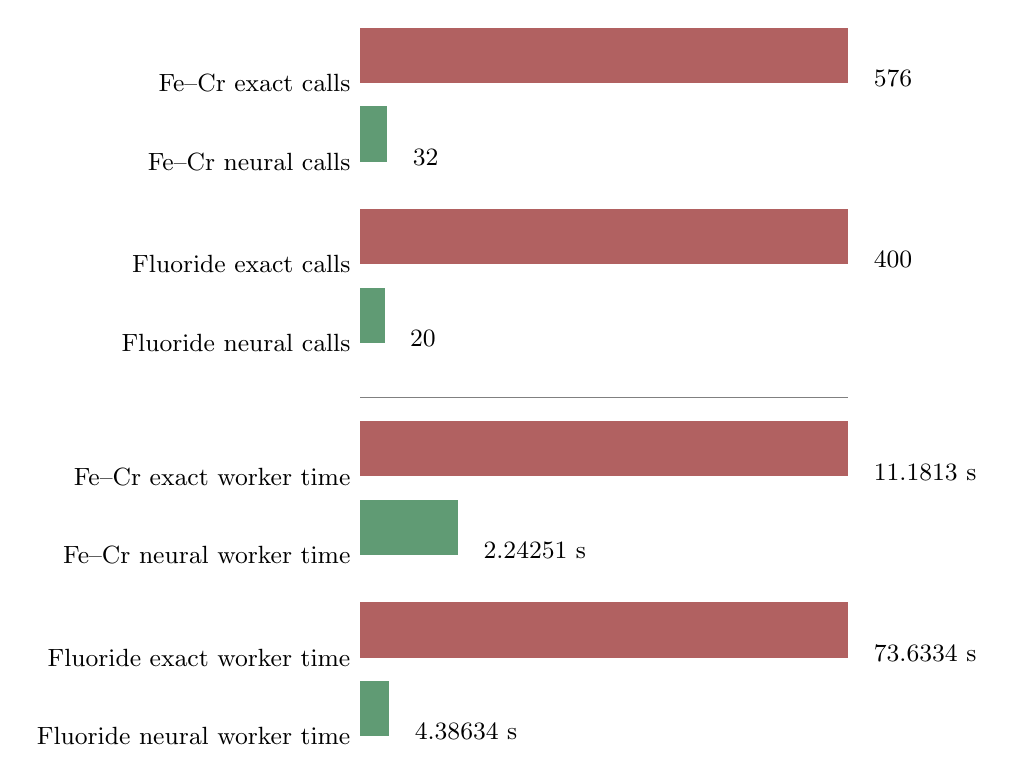
\begin{tikzpicture}[font=\small]
    \def\barheight{7mm}
    \def\fullwidth{62mm}

    \node[anchor=east] at (0,0) {Fe--Cr exact calls};
    \fill[exactred!75] (0,0) rectangle (\fullwidth,\barheight);
    \node[anchor=west] at (\fullwidth+2mm,0.5\barheight) {576};

    \node[anchor=east] at (0,-10mm) {Fe--Cr neural calls};
    \fill[acceptgreen!75] (0,-10mm) rectangle (3.444mm,-10mm+\barheight);
    \node[anchor=west] at (5.444mm,-10mm+0.5\barheight) {32};

    \node[anchor=east] at (0,-23mm) {Fluoride exact calls};
    \fill[exactred!75] (0,-23mm) rectangle (\fullwidth,-23mm+\barheight);
    \node[anchor=west] at (\fullwidth+2mm,-23mm+0.5\barheight) {400};

    \node[anchor=east] at (0,-33mm) {Fluoride neural calls};
    \fill[acceptgreen!75] (0,-33mm) rectangle (3.1mm,-33mm+\barheight);
    \node[anchor=west] at (5.1mm,-33mm+0.5\barheight) {20};

    \node[anchor=east] at (0,-50mm) {Fe--Cr exact worker time};
    \fill[exactred!75] (0,-50mm) rectangle (\fullwidth,-50mm+\barheight);
    \node[anchor=west] at (\fullwidth+2mm,-50mm+0.5\barheight) {11.1813 s};

    \node[anchor=east] at (0,-60mm) {Fe--Cr neural worker time};
    \fill[acceptgreen!75] (0,-60mm) rectangle (12.43mm,-60mm+\barheight);
    \node[anchor=west] at (14.43mm,-60mm+0.5\barheight) {2.24251 s};

    \node[anchor=east] at (0,-73mm) {Fluoride exact worker time};
    \fill[exactred!75] (0,-73mm) rectangle (\fullwidth,-73mm+\barheight);
    \node[anchor=west] at (\fullwidth+2mm,-73mm+0.5\barheight) {73.6334 s};

    \node[anchor=east] at (0,-83mm) {Fluoride neural worker time};
    \fill[acceptgreen!75] (0,-83mm) rectangle (3.693mm,-83mm+\barheight);
    \node[anchor=west] at (5.693mm,-83mm+0.5\barheight) {4.38634 s};

    \draw[gray] (0,-40mm) -- (\fullwidth,-40mm);
  \end{tikzpicture}
  \caption{Measured exact-solve counts and aggregate worker times.  Bar lengths are normalized
  within each case and metric pair, so call-count and time bars are not cross-scaled.}
  \label{fig:performance-bars}
\end{figure}

\subsection{Legacy off-gassing trajectory behavior}

Across the shifted fluoride validation interval, the exact ideal-gas amount decreases from
approximately \(0.3800\) to \(0.2276\), a 40.1\% reduction.  Its fraction falls from
\(8.690\times10^{-3}\) to \(5.249\times10^{-3}\).  The MSFL amount changes more mildly from
\(43.3510\) to \(43.1291\), while its fraction rises from 0.99131 to 0.99475.  This makes the case a
useful off-gassing demonstration: the network resolves a physically meaningful gas depletion
while retaining accurate Gibbs energy and F potential.

The longer source trajectory contains sharp thermodynamic changes near \(x\approx0.219\) and
eventual disappearance of the gas phase near \(x\approx0.5\).  Those regimes were excluded from
the archive.  Extending the present network across them without regime-aware sampling would turn a
successful interpolation problem into an unqualified phase-transition extrapolation problem.

\section{Computational cost and scaling}

\subsection{Training cost}

For \(N_t\) training states, \(N_v\) validation states, \(L\) executed epochs, and
\(N_{\theta}\) parameters, dense forward/backward work scales approximately as
\begin{equation}
  C_{\mathrm{train}}
  =O\left(L(N_t+N_v)N_{\theta}\right).
  \label{eq:training-cost}
\end{equation}
Exact data generation often dominates this small network's training cost:
\begin{equation}
  C_{\mathrm{offline}}
  =N\,C_{\mathrm{GEM}}+C_{\mathrm{train}}.
  \label{eq:offline-cost}
\end{equation}
Offline cost is amortized only when the archive is reused across enough simulation states or
runs.  If database, units, output order, or selected phases change, the digest and metadata checks
correctly prevent that amortization from being obtained by reusing an incompatible model.

\subsection{Runtime cost}

For a worker batch with \(B_e\) eligible rows,
\begin{equation}
  C_{\mathrm{NN,batch}}
  =O(B_eN_{\theta})+O(B_e(d+m)).
  \label{eq:inference-cost}
\end{equation}
The safeguarded total is approximately
\begin{equation}
  C_{\mathrm{runtime}}
  =
  N_{\mathrm{GEM,neural}}C_{\mathrm{GEM}}
  +\sum_{\mathrm{batches}}C_{\mathrm{NN,batch}}
  +C_{\mathrm{IPC}}+C_{\mathrm{MOOSE}}.
  \label{eq:runtime-cost}
\end{equation}
The method is attractive when \(C_{\mathrm{GEM}}\) is large relative to a dense forward pass and
the acceptance fraction is high.  This explains the stronger speedup in the multielement fluoride
case, whose exact GEM workload is much more expensive than the binary BCC case.

Let \(f\) be the fraction of exact application wall time attributable to avoidable GEM work and
\(S_G\) the speedup of that portion.  An Amdahl-style ceiling is
\begin{equation}
  S_{\mathrm{wall}}
  \leq\frac{1}{(1-f)+f/S_G}.
  \label{eq:amdahl}
\end{equation}
Reporting worker time alone therefore overstates application benefit when startup, I/O, mesh
evaluation, or interprocess communication dominates.

\subsection{Worker replication}

With \(p\) workers, model storage is \(O(pN_{\theta})\).  Exact seeds and audit sequences are also
replicated.  If each worker accepts \(n_k\) neural rows, the number of scheduled audits is roughly
\begin{equation}
  N_{\mathrm{audit}}\approx
  \sum_{k=1}^{p}\left\lfloor\frac{n_k}{M}\right\rfloor,
  \label{eq:worker-audits}
\end{equation}
not simply \(\lfloor N/M\rfloor\).  Changing thread or MPI partitioning can therefore change exact
call count while leaving the archive unchanged.

\section{Discussion}

\subsection{Why the two legacy demonstrations succeed}

Both datasets restrict the regression problem to a smooth represented regime.  Fe--Cr has two
independent thermodynamic directions: temperature and binary composition.  The fluoride problem
has more chemical species and a more expensive exact solve, but its training states lie on one
dense trajectory.  In both cases:
\begin{itemize}[leftmargin=*]
  \item logarithmic \(T\) and \(P\) and standardized outputs give numerically balanced inputs and
  losses;
  \item extensive normalization removes total-composition scaling;
  \item the network is overparameterized relative to the low-dimensional sampled map but still
  small in absolute size;
  \item batched inference amortizes C++/PyTorch call overhead; and
  \item exact calls are limited to worker seeds and audits because all queried rows pass bounds and
  invariants.
\end{itemize}

\subsection{Safety model}

The runtime is fail-closed for detectable deployment errors.  A wrong database, element order,
unit system, phase selection, output order, descriptor, or output semantic flag prevents model
initialization.  Out-of-domain and invalid rows execute exact GEM.  A model exception disables the
worker, and an audit error both publishes the exact row and disables future inference.

These mechanisms substantially reduce integration risk, but they are empirical rather than
formal.  Schema 2 closes two important holes: a coordinatewise in-box point must also lie near
training anchors of its classified assemblage, and declared complete fraction groups must satisfy
their coupled sums.  Unexpressed thermodynamic identities can still be violated.  Auditing detects
sampled errors after deployment; it does not prove every unaudited row correct.

\subsection{Comparison with in-situ adaptive models}

The existing local-IDW and KKT-linear methods learn from exact states visited by the current
simulation.  They require no offline archive and can react to a new trajectory, but their
worker-local tables must be populated and their retrieval safeguards add per-state work.  The
neural model moves that learning cost offline and evaluates many rows through matrix operations.
It is most useful for repeated runs over a known operating envelope.

The approaches are complementary:
\begin{itemize}[leftmargin=*]
  \item use exact mode for reference, validation, and unqualified domains;
  \item use a neural archive for a repeatedly traversed, well-sampled regime;
  \item use local-IDW or KKT-linear for online adaptation when offline coverage is unavailable; and
  \item consider a future hierarchy in which neural rejection falls through to an in-situ
  predictor before exact GEM, but only after the simpler single-surrogate prototype is fully
  qualified.
\end{itemize}
The last item is not implemented here; adding it tonight would obscure rather than strengthen the
current evidence.

\subsection{Interpretation of the legacy fluoride demonstration}

The gas-bearing interval remains a useful performance microbenchmark but not a globally valid
reactor chemistry model.  Its seven-dimensional bounding box is constructed from a one-dimensional
curve.  The revised campaign takes the first, more general path: an independently perturbed
multidimensional envelope, unrestricted phase discovery, explicit phase classification, and a
distance-to-data guard.  Until its held-out acceptance gates pass, the legacy timing is not
evidence for the new ten-element fluoride archive.

\section{Guarantees, limitations, and qualification path}

\subsection{What is guaranteed by the implementation}

For a successfully initialized archive:
\begin{itemize}[leftmargin=*]
  \item input and output ordering is checked against metadata;
  \item the database bytes and selected phase configuration are checked;
  \item schema-2 rows outside recorded marginal bounds or calibrated per-assemblage support are
  not inferred;
  \item low-confidence or amount-inconsistent phase labels are not inferred;
  \item nonfinite, scalar-invariant, and declared coupled-invariant failures are not published;
  \item audit rows publish exact values; and
  \item one audit failure disables the responsible worker's neural path.
\end{itemize}
If libtorch is absent, exact and non-neural modes remain available.

\subsection{What is not guaranteed}

The archive does not provide:
\begin{itemize}[leftmargin=*]
  \item a formal uniform error bound over its bounding box;
  \item thermodynamic consistency among independently regressed output columns;
  \item correct behavior at an unseen phase or constituent transition;
  \item extrapolation beyond the sampled temperature, pressure, or composition range;
  \item bitwise equivalence across PyTorch versions or platforms;
  \item load balancing invariant to MOOSE thread/MPI partitioning; or
  \item a production speedup independent of hardware, batch size, and application overhead.
\end{itemize}

\subsection{Recommended next qualification steps}

The remaining evidence-driven path from preliminary implementation to qualification is:
\begin{enumerate}[leftmargin=*]
  \item finish the independently staggered Fe--Cr test grid and report errors separately for
  single-phase interiors, multiphase interiors, and transition-buffer fallbacks;
  \item run the held-out fluoride scan and fail the case if any unlisted phase or species exceeds
  the discovery threshold;
  \item complete the fixed-cost and fixed-accuracy 2/5-element curves locally, followed by the
  9/13/17-element SLURM array;
  \item complete exact and neural replay over identical fresh/depleted NS fields and report
  fluorine-potential maps, iodine distributions/vapor pressures, integrated gas inventory, and
  phase/fallback maps;
  \item archive exact and neural CSV files, full logs, executable digest, source revisions,
  training spec, archive digest, host topology, and environment package lists;
  \item execute the configured repeated timings: quick manifests schedule three repetitions and
  full manifests schedule seven, with mean, median, standard deviation, approximate 95\%
  confidence half-width, aggregate worker time, and end-to-end wall time retained separately;
  \item evaluate a PT2/AOTInductor loader only after the TorchScript scientific contract and
  benchmark archive are stable.
\end{enumerate}

\section{Conclusions}

The implemented capability separates thermodynamic authority from approximation: Thermochimica
generates truth data and remains available for every rejected or audited state, while PyTorch
provides a compact batched approximation only for represented states.  Schema 2 adds the missing
multiphase safeguards: calibrated phase-presence classification, per-assemblage support distance,
trace-output transforms, explicit model-output layout, and coupled fraction invariants.

The revised exact discovery evidence demonstrates that
\code{MSDTC\_41\_fluorides.dat} produces scientifically relevant condensed multiphase behavior in
the chosen ten-element envelope.  The smoke scan found solid LiF, Ni solid, and U solid alongside
MSFL and gas; 7 of 8 states satisfied the MSFL-plus-non-gas requirement.  This is a meaningful
improvement over the original gas-only framing, but it is not yet an accuracy or speed result.

The earlier \(4.99\times\) Fe--Cr and \(16.79\times\) fluoride worker-time results remain recorded
only as legacy smooth-regime measurements.  They do not qualify the new phase-aware studies.
Until the independent multiphase, element-scaling, unseen-output, audit, and NS timing gates pass,
\code{acceleration=exact} remains the production reference and no fluoride-wide acceleration claim
is made.

\section{Relation to prior work and deployment guidance}

Thermochimica's Gibbs-energy formulation and multiphysics motivation are described by Piro
et al.~\cite{piro2013}.  On-demand machine-learning acceleration of equilibrium calculations has
also been demonstrated in reactive-transport settings by Leal et al.~\cite{leal2020}.  The present
work differs in its offline model, embedded archive identity, MOOSE worker-process deployment, and
exact audit/disable policy.

The network is a standard multilayer regression model with the SiLU activation
\cite{elfwing2018} and Adam optimization \cite{kingma2015}.  Its scientific safety does not follow
from the universal approximation capacity of neural networks; it follows from limiting the
represented problem, preserving output semantics, rejecting identifiable mismatches, and retaining
exact GEM.

PyTorch's C++ export documentation marks TorchScript as deprecated and directs new deployment work
toward newer export paths \cite{torchscript}.  AOTInductor provides a C++ deployment route
\cite{aotinductor}, but it should be introduced as a new archive schema with explicit version and
platform provenance rather than substituted invisibly.

\begin{thebibliography}{9}
  \bibitem{piro2013}
  M. H. A. Piro, S. Simunovic, T. M. Besmann, B. J. Lewis, and W. T. Thompson,
  ``The thermochemistry library Thermochimica,''
  \emph{Computational Materials Science}, 67, 266--272, 2013.
  \url{https://doi.org/10.1016/j.commatsci.2012.09.011}

  \bibitem{leal2020}
  A. M. M. Leal, S. Kyas, D. A. Kulik, and M. O. Saar,
  ``Accelerating Reactive Transport Modeling: On-Demand Machine Learning Algorithm for Chemical
  Equilibrium Calculations,''
  \emph{Transport in Porous Media}, 133(2), 161--204, 2020.
  \url{https://doi.org/10.1007/s11242-020-01412-1}

  \bibitem{elfwing2018}
  S. Elfwing, E. Uchibe, and K. Doya,
  ``Sigmoid-weighted linear units for neural network function approximation in reinforcement
  learning,''
  \emph{Neural Networks}, 107, 3--11, 2018.
  \url{https://doi.org/10.1016/j.neunet.2017.12.012}

  \bibitem{kingma2015}
  D. P. Kingma and J. Ba,
  ``Adam: A Method for Stochastic Optimization,''
  \emph{Proceedings of the 3rd International Conference on Learning Representations}, 2015.
  \url{https://arxiv.org/abs/1412.6980}

  \bibitem{torchscript}
  PyTorch,
  ``Loading a TorchScript Model in C++,''
  official documentation, accessed 29 July 2026.
  \url{https://docs.pytorch.org/tutorials/advanced/cpp_export.html}

  \bibitem{aotinductor}
  PyTorch,
  ``AOTInductor: Ahead-Of-Time Compilation for PyTorch,''
  official documentation, accessed 29 July 2026.
  \url{https://docs.pytorch.org/docs/main/user_guide/torch_compiler/torch.compiler_aot_inductor.html}

  \bibitem{vtbthermo}
  Idaho National Laboratory,
  ``MSFR Spatially-resolved thermochemistry model using Thermochimica,'' Virtual Test Bed,
  model documentation, input, depletion CSV, and results, accessed 29 July 2026.
  \url{https://github.com/idaholab/virtual_test_bed/tree/devel/msr/msfr/thermochemistry}
\end{thebibliography}

\appendix

\section{Archive metadata example}

The following abridged example shows the contract shape.  Output descriptors are ordered and
include type-specific selectors.

\begin{lstlisting}[caption={Abridged schema-version-2 archive metadata.}]
{
  "schema_version": 2,
  "archive_type": "thermochimica_neural_torchscript",
  "database_sha256": "1236d1a57bf0f12eea6e0e20d99747b2...",
  "elements": ["Fe", "Cr"],
  "temperature_unit": "K",
  "pressure_unit": "bar",
  "composition_unit": "moles",
  "phase_selection": {"mode": "none", "phases": []},
  "outputs": [
    {
      "type": "chemical_potential",
      "variable": "bcc_cr_potential",
      "phase": "BCC_A2",
      "species": "CR:VA",
      "extensive": false,
      "nonnegative": false,
      "fraction": false,
      "relative_tolerance": 0.001
    }
  ],
  "input_lower_bounds": [1.40198, 0.0, 0.109375, 0.459375],
  "input_upper_bounds": [1.76321, 0.0, 0.540625, 0.890625],
  "phase_gate": {
    "confidence_threshold": 0.99,
    "temperature": 0.79,
    "phases": [{"phase": "BCC_A2", "output_index": 6,
                "presence_threshold": 1e-8}]
  },
  "support": {
    "coordinate_system": "training_standardized_euclidean",
    "assemblages": [
      {"signature": [1], "distance_index": 18, "radius": 0.42}
    ]
  },
  "model_output_layout": {
    "regression_width": 17,
    "phase_logit_offset": 17,
    "phase_logit_count": 1,
    "support_distance_offset": 18,
    "support_distance_count": 1
  },
  "invariant_groups": [
    {"output_indices": [7, 9, 11, 13, 15],
     "target": 1.0, "tolerance": 0.001}
  ],
  "torch_version": "2.10.0",
  "validation_loss": 5.00013e-7,
  "validation_metrics": []
}
\end{lstlisting}

\section{Reproducibility commands}

The trainer can be run directly after an exact CSV has been generated:
\begin{lstlisting}[language=bash,caption={Direct Fe--Cr training.}]
conda run -n ml python \
  modules/chemical_reactions/benchmarks/thermochimica_neural/train_thermochimica_nn.py \
  --data /persistent/results/fe_cr_training.csv \
  --validation-data /persistent/results/fe_cr_validation.csv \
  --spec modules/chemical_reactions/benchmarks/thermochimica_neural/fe_cr_multiphase.json \
  --output /persistent/results/fe_cr.pt
\end{lstlisting}

The qualification driver generates exact data, trains, and executes the requested campaign:
\begin{lstlisting}[language=bash,caption={Quick qualification commands.}]
conda run -n ml python \
  modules/chemical_reactions/benchmarks/thermochimica_neural/qualification.py \
  fe_cr --tier quick --workdir /persistent/results/fe_cr

conda run -n ml python \
  modules/chemical_reactions/benchmarks/thermochimica_neural/qualification.py \
  elements --tier quick --workdir /persistent/results/elements

conda run -n ml python \
  modules/chemical_reactions/benchmarks/thermochimica_neural/qualification.py \
  fluoride --tier quick --workdir /persistent/results/fluoride

conda run -n ml python \
  modules/chemical_reactions/benchmarks/thermochimica_neural/qualification.py \
  ns --tier quick --workdir /persistent/results/msfr_ns

conda run -n ml python \
  modules/chemical_reactions/benchmarks/thermochimica_neural/plot_qualification.py \
  --workdir /persistent/results
\end{lstlisting}

A publication-quality result directory should retain:
\begin{lstlisting}[caption={Minimum persistent result archive.}]
exact.csv, neural.csv             state-by-state outputs
exact.log, neural.log             complete MOOSE output and telemetry
training_spec.json                immutable trainer configuration
surrogate.pt                      deployed archive
surrogate.validation.json         embedded metadata in readable form
sha256sums.txt                    archive, database, executable, and inputs
source_revisions.json             MOOSE and Thermochimica revisions
environment.txt                   Python, PyTorch, compiler, and libtorch
timings.csv                       all exact/neural repetitions
host.json                         CPU, memory, OS, affinity, thread and MPI layout
figures/*.pdf, figures/*.png      deterministic campaign visualizations
\end{lstlisting}

\section{Focused test matrix}

\begin{longtable}{L{0.32\textwidth}L{0.28\textwidth}L{0.32\textwidth}}
  \caption{Prototype capability-gated tests and expected behavior.}
  \label{tab:tests}\\
  \toprule
  Test & Perturbation & Required result \\
  \midrule
  \endfirsthead
  \toprule
  Test & Perturbation & Required result \\
  \midrule
  \endhead
  Successful inference &
  Compatible archive and in-domain states &
  Ordered predictions, neural hits, and reduced exact calls. \\
  Metadata mismatch &
  Wrong element order, database digest, unit, phase selection, or output &
  Worker initialization fails with a specific archive/configuration error. \\
  Out-of-domain fallback &
  At least one canonical coordinate outside bounds &
  Row is exact and out-of-bounds telemetry increments. \\
  Outside-support fallback &
  In-box coordinate beyond the classified assemblage radius &
  Row is exact and support-rejection telemetry increments. \\
  Phase-boundary fallback &
  Confidence below 0.99 or phase amount contradicts its label &
  Row is exact and phase-rejection telemetry increments. \\
  Nonfinite/model failure &
  Archive returns NaN or invalid shape &
  Prediction is not published; exact fallback is used and worker inference is disabled on
  forward-level failure. \\
  Invariant rejection &
  Negative/scalar-invalid output or incomplete phase/element sum &
  Row is exact and invariant-rejection telemetry increments. \\
  Audit disablement &
  Deliberately inaccurate but finite archive &
  Audited row publishes exact; failure is reported; subsequent rows in that worker are exact. \\
  Multithread execution &
  Four MOOSE threads/workers &
  Independent CPU models complete without Fortran or PyTorch state races. \\
  Regression compatibility &
  Existing exact, local-IDW, and KKT tests &
  Behavior remains unchanged when neural mode is not selected. \\
  \bottomrule
\end{longtable}

\end{document}
